\documentclass[
class = book,
zihao = -4,
font = noto,
paper = a4paper,
openany
]{easybook}
\PassOptionsToPackage{monochrome}{xcolor}
\usepackage{xju}
\newcommand{\ti}{Ti6Al4V}

\begin{document}
	\hypersetup{pdftitle=热处理温度及冷却速度对Ti6Al4V组织和力学性能的影响,pdfauthor=田欣洋,pdfsubject={材料科学,金属学,钛合金},pdfkeywords={热处理,固溶,时效,组织},pdfstartview=FitB}
	\maketitle
	\frontmatter*[roman]
	\includepdf{附件/封面与声明}
	\includepdf{附件/田欣洋 新疆大学2023届本科毕业论文(设计)任务书 }
	\begin{abstract}
	\ti 合金又名TC4合金,拥有较好的塑韧性、耐热性、成形性、耐蚀性等,
%	其使用量已占钛合金使用总量的75$ \% $~85$ \% $,也是大多数高强钛合金的基础,被誉为钛合金中的“王牌合金”,
	在机械、军事、航空航天等领域获得了极为广泛的应用。但TC4合金存在着硬度低、摩擦磨损系数高、耐磨性能差等缺点,制约了其进一步的应用。结构决定组织,组织决定性能。合金的显微组织显然不能轻易被各种冷塑性变形所改变,而热处理恰恰具有这种控制结构、组织的能力。不同的热处理制度会形成不同的组织,进而引起性能的差异。对Ti6Al4V合金而言,常规处理方式得到的合金存在着强硬度偏低、摩擦性能差等缺点,经过调研\ti 合金近几十年的研究可以发现:固溶+时效处理是一种比较理想的强化手段,可以通过调控合金的显微组织,从而大幅改善合金的强度、硬度与耐磨性。

	本文通过对比九个不同固溶-时效处理工艺参数后得到的Ti6Al4V合金,分析了不同参数下处理Ti6Al4V合金的力学性能,旨在进一步确定TC4合金的最佳固溶温度、时效温度、时效时间等参数,为实际工程应用提供参考。 本文全面系统地描述了950 ℃附近固溶处理、550℃附近时效处理所得的Ti6Al4V合金在室温下$ 10~240 N $施加载荷范围内的力学性能与组织特征。得到了力学性能优良的热处理后\ti 合金所处的工艺参数范围。并结合金相特征和电子显微镜分析测试结果,通过分析合金微观组织特征和力学性能变化,探索固溶体组织转变的机理。主要研究成果如下
%	\footnote{{\color{red}\faBan} 以下几点为胡诌,待实验结束后再整理之!}:
	\begin{enumerate}
		\item (\text{\color{blue}从热处理制度})在950℃进行固溶、550℃进行时效处理时可以得到合金最佳的力学性能。
		\item (\text{\color{blue}从微观组织})冷却速率越高,得到组织所含$ \beta  $相含量越多,综合性能越好。
		\item (\text{\color{blue}从转变机理})时效时间越久,亚稳定$ \beta $相分解的就越充分,得到的组织性能更好。
	\end{enumerate}
	\keywords{热处理;固溶;时效;组织;钛合金;工艺}
	\end{abstract}

	\tableofcontents
	\mainmatter*

	\pagestyle{Xju}
	\chapter{绪论}
\section{钛合金的特点}

钛(Titanium),原子序数为22,最早于1791年由格雷戈尔在英国康沃尔郡发现,具有比强度高、耐高温、生物相容性好、化学性质性质稳定等明显优于传统金属的特性而备受重视。钛及钛合金常用来制造飞机、火箭等航天机械,一直以来都是航空航天工业的“脊柱”之一,被誉为“太空机械”\cite{XJYS200102014}。
与纯钛一起发展起来的钛合金也毫不逊色,凭借其强度更高、耐腐蚀、耐高温的特性,尤其是在机械制造、航天、化工、军工等领域,钛合金所占比重更大,是在各种合金元素的基础上添加纯钛而形成的合金\cite{HSJJ202109005}。钛合金具有密度小,强度高的显著特点,相较于高强度钢而言,不仅强度相差无几,而且还具有更大的比强度\cite{hardestyMetalsHandbookNinth1982},如\ref{sec:bqd}所示。
\begin{table}[htbp]
	\centering
	\caption{不同合金比强度比较表}
		\label{sec:bqd}
	\begin{tabular}{ccccc}
		\toprule
		{合金} & {镁合金} & {铝合金} & {高强钢} & {钛合金} \\
		\midrule
		比强度 & 16 & 21 & 23 & 29 \\
		\bottomrule
	\end{tabular}
\end{table}

钛合金的特点如下\cite{1997titanium}:
\begin{enumerate}
	\item 熔点高。钛的熔点为1660℃,比铁的熔点还高出120℃左右。此外,在钛中加入铝、锆、锡等稳定元素后,可以提高合金热强性。
	\item 弹性模量低,屈服强度高。综合性能优良
	\item 耐磨性、耐腐蚀性好。钛表面易生成致密的氧化层,在氧化性或中性介质中有较强的耐腐蚀能力。
%	\item 化学活性高。当钛加热到500℃以上时,氧化膜变得稀松且易脱落,在熔融状态下,极易发生自然。
%	\item 特殊性能多。某些类型的钛合金还具有储氢、超导、低阻尼性,生物相容性、形状记忆 、 超弹 、高阻尼等特殊功能。
\end{enumerate}

\subsection{钛合金的国内外发展}
%钛合金的发展充满曲折。从钛元素的发现(1791)到第一次制得较纯的金属钛(1910)经历了120年的历程。又由实验室第一次获得纯钛(1940)到首次进行工业生产,又花费了近30年的时间。
%钛在自然界中主要以钛矿石的形式存在,如钛铁矿、金红石(TiO2)等,需要进行精炼(refining)才能获得纯金属。起初,钛的提取是通过高温还原法,但这种方法费时费力,成本高昂。直到了二十世纪四十年代,一种利用氯化钛矿与氯气进行反应来制备四氯化钛,然后通过还原反应(比如Na、Mg等)来得到纯钛的精炼工艺方法终于以其低廉的成本、高效的回收率得到了广泛的商业化应用。
%
%第二次世界大战之后,世界上许多国家都开始意识到钛工业的重要性,钛工业在数年间便迅速发展成为航空、航天、军事等领域的关键材料。1954年,美国成功研发出Ti-6Al-4V合金,该合金在耐热性、强度、塑性、韧性、耐蚀性和生物相容性等方面均达到较高水平,凭借性能上的优势,\ti 迅速成为钛工业的主要合金,现已占据全部用钛量的50%以上,甚至可以说,许多其他型号钛合金不过是Ti-6Al-4V的改良版而已\cite{COLO200102000}。

钛工业的发展历程可谓是一波三折,但是在经历了长达120年的艰难曲折之后,钛工业终于在二十世纪四十年代迎来了重大突破。钛元素虽然在自然界中主要以钛矿石的形式存在,但是经过提炼和精炼处理,可以得到纯金属钛。而最初的高温还原法虽然是提取纯钛的一种方法,但费时费力成本高昂,因此并不实用。直到利用氯化钛矿与氯气进行反应制备四氯化钛的方法被发明,才真正实现了纯钛的精炼,并且该工艺方法具有低廉的成本和高效的回收率,因此得到广泛的商业化应用。

二战之后,世界上的许多国家开始重视钛工业的发展,将其作为航空、航天、军事等领域的关键材料。其中,1954年美国成功研发出的Ti-6Al-4V合金成为了钛工业的主要合金之一。该合金在许多方面的性能均达到了较高水平,迅速成为了主流的钛合金,甚至许多其他型号钛合金不过是对Ti-6Al-4V的改良版本。目前,Ti-6Al-4V已经占据了全部用钛量的$ 50\% $以上\cite{COLO200102000}。


我国的钛工业发展起源于20世纪50年代,在六七十年代,我国成为了全球第四个建立完整钛工业体系的国家。21世纪以来,我国钛工业经历了高速发展阶段,钛工业产量已经连续多年位居全球首位。目前,我国的海绵钛产量占全球比重的$ 60\% $以上,而钛加工材的产量也在稳步增长。在消费端,作为钢铁、航空航天等诸多高端领域重要的原材料,钛产品的需求量也在快速增长\cite{JSTB202209001},无论是在生产还是在加工领域均保持在世界前列\cite{TGYJ200405004}。

目前,我国的钛产品消费正在逐步提升,并且处于上升期。在工业、航空航天、海洋船舶和体育休闲等中高端领域,钛材料的需求量平均增长约$ 20\% $左右,显示出了巨大的市场潜力。不过,疫情对医疗行业的影响仍在,钛材料在医疗行业中的需求量有所减少,但是电力和制盐等行业仍有小幅增长。总体来看,整个钛产品市场的盈利水平也有所改善\cite{BJKY202204004}。
%--------------------
%-------------------
%------------------
%------------------
%------------------

此外,近年来计算机技术的发展也为钛工业带来了新的发展机遇。计算机模拟技术用于优化钛合金的生产工艺,显著提高了产品质量。邵一涛等人利用BP人工神经网络的方法,构建了TC17钛合金组织和性能之间的关系模型,解决了传统BP人工神经网络的过拟合问题,从而获得更高的预测精度\cite{BP};%史延沛、罗皎等人通过将有限元法与 Yada 微观组织模型结合起来,以位错密度速率为内状态变量,模拟分析出了 TC4 合金在锻造过程中初生$\alpha$晶粒的变化规律。
在未来,随着人工智能、ChatGPT等技术的不断落地,钛工业也将迎来更多新的机遇和挑战\cite{Moni}。人工智能可以为钛工业提供更高效、更精准的技术支持。在技术咨询、产品设计、材料选择、生产流程等方面,人工智能还可以根据用户的需求和特定的业务场景,进行精准的语义理解和模型训练,提供针对性的解决方案和建议。这将极大地提高钛工业的生产效率、产品质量和市场竞争力,帮助钛工业实现数字化、智能化升级,对于钛工业的发展具有重要的推动作用。
\subsection{应用领域}

\begin{itemize}
\item  在航空航天领域,大型客机的设计制造推进迅速,同时军用飞机也在不断更新换代,因此全球钛合金的需求量也在急速增长。
\item  在医疗健康领域,钛合金材料有着良好的生物相容性,可以降低人体对植入物的排斥反应和感染风险,因此广泛用于人工关节、牙科种植体和其他医疗设备的制造。
\item  在汽车制造领域,高级车型的制造中广泛采用了钛合金零部件,以降低整车自重,提高燃油效率和汽车的运行性能。此外,钛合金耐腐蚀性好也能延长汽车零部件的使用寿命。
\item  在建筑工程领域,钛合金广泛应用于大型建筑的外墙幕墙、顶棚和立面系统中。这种材料具有优秀的耐候和抗腐蚀性能,可抵御各种恶劣气候的侵蚀,并且具有高度的可塑性和装饰性,可以为建筑带来更加优美的外观效果。

\end{itemize}
\section{钛合金的分类}
\label{sec:1.1}
因为纯钛的强度较低,限制了其在工业生产中的应用范围。钛合金是通过在纯钛中添加一些合金元素来提高其强度、耐腐蚀性等性能而形成的。常用的合金元素有铝、钒、锆、锂、铁、铜、镍等,通过调整元素配比和控制制备工艺,可以获得适合不同领域应用的各种高性能钛合金材料。

工业钛合金的主要合金元素为铝、钒、钼三种,此外还有Cr、Mn、Fe、Cu、Sn、Zr、W等元素组成,根据不同的合金元素对钛多晶型转变温度的影响可以分为三类:稳定𝛼相的元素、稳定𝛽相的元素和中性元素。

可根据不同合金元素对钛多晶型转变温度的影响,分为三大类:$\alpha$稳定元素、$\beta$ 稳定元素、中性元素,形成的四种类型的相图示意图如图1.1所示。
\begin{figure}[h!]
	\centering
	\includegraphics[width=0.9\linewidth]{pic/01}
	\caption{合金元素对钛合金相图的影响示意图}
	\label{fig:01}
\end{figure}

工业上一般根据$\beta$相稳定元素系数$K_{\beta}$来划分不同的合金元素,$K_{\beta}$是指合金中各$\beta$稳定元素与各自的临界浓度的比制之和,即:
\begin{equation}
K_{\beta}=\frac{ C_{1} }{C_{k1}}+\frac{ C_{2} }{C_{k2}}+\frac{ C_{3} }{C_{k3}}+\cdots+\frac{ C_{n} }{C_{kn}}
\end{equation}
根据 $\beta$ 相稳定系数划分合金类型为: $\alpha$ 型合金 、近 $\alpha$ 型合金 、$\alpha+\beta$ 型合金、近 $\beta$ 型合金、$\beta$ 型 合金。
%
%\paragraph{(1)$\alpha$型($K_\beta$ 为 $0 \sim 0.07$)}
%经退火处理后,$\alpha$型钛合金的组织通常存在单相的$\alpha$固溶体,或者以含微量金属化合物的$\alpha$固溶体的形式存在。其主要合金元素包括铝、锡、锆等$\alpha$稳定元素,以及钒、钼、铌等中性元素,各个元素都可以起到固溶强化的作用,因此这些元素都被广泛地应用于钛合金的制备中。
%
%常用的$\alpha$型钛合金包括TA2(工业纯钛)、TA9(Ti-0.2Pb)等。
%
%$\alpha$型钛合金的$\beta$相转变温度较高,因而具有良好的热强性、高温稳定性。焊接性性能好,并在高温环境下具有极好的组织稳定性和抗蠕变性能,在低温环境下也依然保持良好的延展性,因而适合制作各种飞行器形状复杂的外层板材。但它对热处理和组织类型不敏感,故不能采用热处理的方式强化其组织\cite{TiandAl}。
%\paragraph{(2)$\beta$型($K_\beta$ 为 > $ 2.8 $)}
%$\beta$型钛合金主要包含钒、钼、铌、钽等$\beta$相稳定元素,若在合金中加入少量的铝、锆、锡等元素,则可以提高$\beta$型钛合金的塑性,并且改善其热稳定性。这些合金元素的加入可以控制合金的相转变温度,使其具有更加优异的力学性能和高温耐久性。
%常见的$\beta$型钛合金有TB2(Ti-5Mo-5V-8Cr-3Al)、TB6(Ti-10V-2Fe-3Al)、TB7(Ti-36Mo)等。
%
%与$\alpha$型、$\alpha+\beta$型钛合金相比,$\beta$型钛合金的显微组织通常更粗大。该合金具有良好的冷成形、冷加工性能,较好的淬火态塑性以及可焊接性。但是,亚稳态$\beta$型钛合金的热稳定性较差。$\beta$型钛合金中含有较高的$\beta$稳定元素,主要分为稳定$\beta$型钛合金和亚稳定$\beta$型钛合金。稳定$\beta$型钛合金在平衡状态下全部由稳定的$\beta$相组成,经热处理后不易产生变化。
%\paragraph{(3)$\alpha$+$\beta$型($K_\beta$ 为  $0.25 \sim 1.0$)}
%经过退火处理的$\alpha+\beta$型钛合金在室温下具有不同比例的$\alpha$和$\beta$相组织,其锻造和轧制等加工成型性能比$\alpha$型、$\beta$型钛合金更加优异。合金中除了含有定量的铝元素外,还含有少量的其他元素,可以通过适当的热处理方法对$\alpha+\beta$型钛合金进行组织强化。其强度和淬透性随着$\beta$相稳定元素含量的增加而提高。
%
%最常用的$\alpha$+$\beta$型钛合金包括TC4、TC6、TC12等,其中TC4钛合金(等轴马氏体型两相合金)作为做早被应用的钛合金,该合金以其优越的性能占据了钛工业的大量市场,现在占到 Ti 合金总产量的 50$ \%  $, 占到全部Ti 合金加工件的95$ \% $ 。
%
%从成分上来看,这类钛合金中的合金元素基本上是以铝为主要合金元素,$\beta$稳定化元素为辅助元素。这使得$\alpha$+$\beta$型钛合金组织变动的余地较为灵活,性能变动范围大,可以满足各种应用场合及工况要求\cite{TiandAl}。
\section{钛合金的显微组织}
钛合金的性能是由显微组织的形态决定的, 甚至组织上的细微差异有时都会得到迥然不同的力学性能表现,显微组织形态则与元素含量、加工方式和热处理方式等环节息息相关。钛合金的基本组织有两种:低温的$\alpha$相和高温$\beta$相,两者特点如\ref{sec:alphaandbeta}所示:

\begin{table}[htbp]
	\centering
	\caption{钛合金基本组织的对比}
	\label{sec:alphaandbeta}
	\begin{tabular}{ccc}
		\toprule
		 特点&$ \alpha $相&$ \beta $相\\ \midrule
		 结构类型 & 六方最密堆积结构(HCP) & 体心立方结构(BCC) \\
		 原子排列 & 沿c轴密排 & 八面体最紧堆积结构\\
		 密度 & 4.43g/cm³ & 4.51g/cm³ \\
		 成分 & Ti-6Al-4V、Ti-6Al-2Sn-4Zr-2Mo等 & Ti-12Mo-6Zr-2Fe等 \\
		 形成温度 & 900℃-1000℃ & 700℃-800℃ \\
 		 稳定温度 & <882.5℃ & 882.5℃熔点 \\
 		 变形难易 & 困难 & 容易 \\
 		 滑移系 & 四个 & 十二个 \\
		 成形能力 & 较差,易发生晶粒长大、裂纹 & 易于变形,加工性能较好 \\
		 机械性能 & 强度和延展性能较好 & 韧性与热强性好 \\
		 耐腐蚀性能 & 良好 & 较差,易于发生点蚀、坑蚀等 \\
		\bottomrule
	\end{tabular}
\end{table}

TC4合金在加热到$ \beta $相变点以上后完全$ \beta $相化,但由于TC4合金内$ \beta $相稳定元素较少,体心立方的高温$\beta$相几乎不可能随着冷却过程保留到室温。$\beta$相在冷却过程中发生多种固态相变,形成多种多样的组织:随着温度降低,$\alpha$相以片状形态从原始$\beta$晶界析出。这种片状组织主要由相互交错的类似于珠光体一般的片层$\alpha$相与片层$\beta$相构成,称之为$\beta$转变组织。若合金在$\alpha+\beta$两相区状态下受到足够大的塑性变形,片状组织会把塑性变形产生的能量通过再结晶球化的方式再利用,得到形状规则的等轴组织。

根据转化后$\alpha$相的不同形态,TC4($\alpha+\beta$型)钛合金的显微组织大致分为四类:初生等轴组织、双态组织、网篮组织和魏氏组织。各个组织的基本特点如下:
\begin{figure}[h!]
	\centering
	\includegraphics[width=0.7\linewidth]{pic/四种典型组织}
	\caption{四种典型组织(a)等轴组织;(b)魏氏组织;(c)网篮组织;(d) 双态组织}
	\label{fig:classic}
\end{figure}

\begin{itemize}
	\item 	\textbf{等轴组织}:在充分的塑性变形和再结晶退火后可以形成等轴组织。特点是$ \beta $基体上分布着等轴状的$ \alpha $相,疲劳强度高,具有良好的塑性,热稳定性。缺点是断裂韧性、持久强度差。
	\item 	\textbf{网篮组织}:合金在 $\alpha+\beta$ 两相区的塑性变形量不太大时形成网篮组织。其特点是晶内$ \alpha $片短小弯曲,在$ \beta $相晶粒周围分布,呈现出网篮状的形状,具有较高的疲劳强度和蠕变强度,塑韧性好。
	\item 	\textbf{双态组织}:双态组织与等轴组织类似,双态组织具有较高断裂韧性,疲劳裂性能好。等轴 $\alpha$ 含量在 $20 \%$ 左右的双态组织具有强度高、塑韧性好的综合力学性能,但高温性能较差。
	\item 	\textbf{魏氏组织}:在较高温度的 $\beta$ 区加热或变形量不够,时可以形成。如图\ref{fig:classic}(d)所示组织中 $\beta$ 晶粒的晶界比较完整,晶粒内有呈粗片状规则排列的长而平直的 $ \alpha $相,其断裂韧性、持久强度、蠕变性能好,但是塑性较差,疲劳强度低、热稳定性差,热处理时尽量避免该组织的形成。
\end{itemize}

\section{钛合金的相变}
钛合金的相变非常复杂,大体可以分为:同素异晶转变、共析转变、有序化转变、亚稳相分解、马氏体相分解等。

%	众多研究者已将钛合金的相变类型绘制成了一个表格:
%	\begin{table}[htbp]
	%	\centering
	%	\label{sec:change}
	%	\caption{相变过程}
	%		\begin{tabular}{ccc}
		%			\hline
		%			编号 & 相变 & 过程 \\ \hline
		%			I & 淬火过程中$\beta$相的分解 & (1)钛的马氏体:$ \beta $ 	o $\alpha^{\prime}$ , $\alpha^{\prime\prime}$\$ \\ \hline
		%	~ & 淬火过程中$\beta$相的分解 & (2)无热\$$\backslash$omega\$相:\$$\backslash$beta $\backslash$to $\backslash$omega\_\{$\backslash$text\{无热}} +$\backslash$beta\$ \\ \hline
%II & 等温转变中$\beta$相的分解 & (1) \$$\backslash$beta($\backslash$beta+$\backslash$alpha)$\backslash$to a\^\{\prime\prime},a\^\{\prime\prime}$\backslash$text\{富},a\^\{\prime\prime}$\backslash$text\{贫}\$ \\ \hline`
%~ & 等温转变中$\beta$相的分解 & (2) \$$\backslash$beta\^\{\prime}$\backslash$beta$\backslash$text\{富},$\backslash$beta$\backslash$text\{贫}\$ \\ \hline
%III & 残余$\beta$相分解 & (1)      相离析: \$$\backslash$beta\_\{$\backslash$text\{残}} $\backslash$to $\backslash$beta\^\{\prime}+$\backslash$beta\$ \\ \hline
%\end{tabular}
%\end{table}

在各种类型的钛合金中,$\alpha+\beta$钛合金的用途最为广泛,在纷杂的钛合金相变中,可根据亚稳定状态相组成将其分为3类 :稳定$\beta$型钛合金 、 亚稳定$\beta$型钛合金和近$\beta$型钛合金。

通过快速冷却$\beta$相可以使之保持在亚稳定状态,但在一定温度下亚稳态会逐渐分解以降低系统的自由能。亚稳定$\beta$相在分解时,视$ \beta $稳定元素的占比不同,亚稳$ \beta $相可以分解成$ \omega $相、$ \alpha^{\prime} $相、$ \alpha^{\prime\prime} $相等,从而得到不同性能的合金组织。
%之所以会出现这种渐进式分解,是因为成分范围较广的钛合金虽然可以通过快速冷却相保持在亚稳定状态,然后在高于室温的温度下逐渐分解,但由于密排六方点阵的的$\alpha$相难以在体心立方点阵的相基体中生核内,因此在温度不太高的情况下,有些中间分解产物更容易产生核。因此,亚稳定相不能直接分解形成平衡的相,而是由生成的某些中间分解产物(或称过渡相),经过某些中间分解过程,再转变为平衡的$\alpha$相。至于哪一种过渡相的形成,则要看制热的温度,以及其中的合金成分等因素而定。

依据钛合金的这种特性,可以根据不同的加热温度、冷却速度来进行处理以得到想要的微观组织,此即本设计采用固溶时效来强化合金性能的理论基础。
% 内容删减第一弹
%最常见的过渡相是等温相和$\beta$’相。在500℃范围内加热时,亚稳定$\beta$相的分解过程为:
%\begin{enumerate}
%	\item  $\beta$亚稳→$\beta$'+$\beta$→a\prime\prime+$\beta$→a+$\beta$
%	\item  $\beta$亚稳→$\beta$'+$\beta$→ω+$\beta$→a+$\beta$
%\end{enumerate}
%
%\subsection{马氏体相变}
% 钛合金自高温快速冷却时, 视合金成分不同, $\beta$ 相可转变为马氏体 ( $\alpha^{\prime}$ 或 $\left.\alpha^{\prime \prime}\right) 、 \omega$ 相或过冷 $\beta$ 相。在快速冷却过程中, 由于从 $\beta$ 相转变为 $\alpha$ 相的过程来不及进行, $\beta$ 相将转变为成分与母相相同、晶体结构不同的过饱和固溶体, 即马氏体。
%
%
% 我们知道马氏体转变是一种切变相变。在钛合金中发生马氏体转变时, $\beta$ 相中的原子作集体的有规律的近程迁移, 迁移距离较大时, 形成六方 $\alpha^{\prime}$ 相; 迁移距离较少时, 形成斜方 $\alpha^{\prime \prime}$ 。当 $\beta$ 相中的合金元素含量较少时, 原子位移较大, 点阵改组进行到底, 得到密排六方 $\boldsymbol{\alpha}^{\prime}$ 相; 当合金元素含量较大时, 点阵改组受到阻碍, 停留在某一中间阶段, 即形成斜方点阵 ( $\alpha^{\prime \prime}$ 相)。
%
%\subsection{ ω相变}
%合金成分在临界浓度$C_0$ 附近的合金从高温淬火后 , 将在合金组织中形成一种ω相。ω相可以根据组织分为两类——无热ω相与等温ω相。
%
%\begin{enumerate}
%	\item 无热ω相:当$\beta$合金元素的成分范围达到某一临界值时,合金在$\beta$相区淬火可以得到ω相。其特点是尺寸小,硬度大,脆性极大,会使材料的塑韧性急剧降低,当其含量达到80$ \% $时,合金就会失去宏观塑形。可以通过改变化学成分或者回火工艺予以控制。
%	\item 等温ω相:在淬火得到的亚稳定$\beta$相后,在随后的时效过程中,会出现$\omega \to \beta$转变,时效温度一般在100~500℃之间,相对于无热ω,$\beta$相分解为等温ω相的速度最快。其尺寸较小晶粒密度大,有方形和椭球形状两种形态,其含量越多,合金的硬度越高,塑韧性越差,当含量大约为50$ \% $时合金的综合性能较好。
%\end{enumerate}
%
%\subsection{$\alpha$相的形成}
% 在相分离和ω相变不能出现的高温时效过程中,亚稳$\beta$相可以直接转变为$\alpha$相,进而转变为$ 1\alpha $和$ 2\alpha $两种相
%
%%\begin{enumerate}
%%	\item  在位错及亚晶界上直接形成$\alpha$相;
%%	\item  经过过渡相形成a相
%%	\item  $\beta$→$\beta$'(bcc,贫溶质)→1$\alpha$和2$\alpha$;
%%	\item  $\beta$→ω(hcp,贫溶质)→l$\alpha$和2$\alpha$。
%%\end{enumerate}
%其中,1$\alpha$相为片层状,2$\alpha$为透镜状,但两者的晶体结构并无区别。
%在$\beta$相的时效转变中,有可能生成$\beta$'、ω、1$\alpha$和2$\alpha$相沉淀。$\beta$相对合金的强度无明显改善,相虽能强化合金,但会强烈降低合金的韧性。因此工业上的$\beta$合金都设计成使$\alpha$相(1$\alpha$和2$\alpha$)作为基体中的硬化沉淀相,合金的强度则由时效形成的$\alpha$相粒子尺寸、形状及体积分数控制。有实验数据表明,当合金中出现非共格的、有较大体积分数的、尺寸较大的2$\alpha$型沉淀时,合金将有良好的综合性能。


%\section{钛合金组织分析方法}

\section{\ti 合金热处理研究进展}
TC4钛合金一般利用亚稳$  \beta$相的分解,得到不同的组织来实现组织的强化,近些年来国内对于\ti 合金的研究,在TC4钛合金热处理工艺上也取得了较多成果\cite{guokaiTC4taihejinrechuligongyideyanjiuxianzhuangjijinzhan2021},热处理工艺主要是:固溶处理、时效处理

\begin{enumerate}
	\item 固溶处理:实施固溶处理工艺,是为了得到使$ \alpha $相以等轴、片状的形式存在,初生等轴$\alpha$相能够让合金的力学性能得到综合性的提升,但是会导致塑韧性有所下降\cite{gurong2002}。
	\item 时效处理:时效处理通过控制亚稳$ \beta $相的分解,来实现TC4钛合金在力学的性能上得到更好的提升。研究\cite{luyuanyuanShixiaochuliduiTC4taihejinweiguanzuzhihelixuexingnengdeyingxiang2019}发现,次生的$\alpha$相体积分数在TC4钛合金中,会对屈服强度产生很大的影响。在条件相等的情况之下,时效温度越低组织越小,时效温度高低组织越大。
	\item 深冷处理:深冷处理是深冷处理是一种通过降低温度增强钛合金强度和韧性的处理方法。使原始的$\beta$相转变成$\alpha^{\prime}$相以减少残余应力,以对金属内部的组织进行改善,从而使TC4钛合金的塑韧性得到提高。
\end{enumerate}


\section{研究背景意义与研究内容}
\subsection{研究意义}
\ti 合金具有比强度高、生物相容性好、耐热、化学稳定,等优异特点,在宇航、车辆制造业、医药保健行业等方面获得了应用,是目前使用最为普遍的钛合金。但由于其室温塑性比较小,热加工硬化力不足,冷加工工艺成型比较困难,限制了其更大的应用范围。目前的科学研究中,提高TC钛合金室温塑性的方法主要为加入合金元素、剧烈塑性变形法以及相变热处理。前二类处理工艺对合金的塑性提高效果很好,但是生产成本比较高\cite{miao},而第三种热处理方法则工艺简单,成本低,是提升TC4合金性能的不二之选。

不同的热处理工艺互相组合可以对合金产生更好的强化效果,现阶段工业上常采用\cite{zhoukaixiangJiyushenlengchulidenanjiagongcailiaoqiexiaotexingyanjiu2022}:淬火+时效;固溶+时效;双重固溶+时效;固溶+双重时效;时效+冷轧+低温氮化等,其中固溶+时效处理是应用最为广泛的一种热处理工艺组合。此外还有通过添加一定成分的铁元素进行强化的方法\cite{yuliaoMicrostructuralStrengtheningToughening2022}。但是目前对于固溶+时效处理方法的最佳工艺参数一直没有定论,本设计的目的就是确定\ti 合金最佳的固溶+时效热处理工艺参数,并分析参数对于合金组织与力学性能的影响。

\subsection{研究内容}
本设计通过对TC4钛合金进行多种不同工艺参数的热处理,来重点研究不同固溶温度和冷却方式、时效的温度和时间下,TC4合金显微组织与力学性能的变化规律,也探讨了固溶温度过高对塑性的不良影响,对于解决现有钛合金加工相关的瓶颈问题具有一定借鉴意义,希望可以为实际TC4钛合金的热处理生产工艺提供一些依据。本文研究的主要内容是:
\begin{enumerate}[itemindent=1em]
	\item[(1)] 研究了 相变点以下、$ \alpha+\beta $两相区、相变点以上,三个区域进行固溶处理时温度、冷却方式对于组织形态、初生等轴 $ \alpha $相分布的影响。
	\item[(2)] 研究了不同时效温度对于合金组织、力学性能的影响。
	\item[(3)] 研究了魏氏组织对于合金塑性的影响,并分析了固溶温度过高引起的组织、力学性能变化机理。
\end{enumerate}


	\chapter{热处理实验}
\section{TC4型钛合金的热处理工艺}
由~\ref{sec:1.1}可知,钛合金可以通过各种各样的相变过程来得到不同的组织结构。因而可以设计适宜的热处理工艺参数,来获得具有高强度的显微组织,由此实现\ti 合金力学性能和工艺性能的改善。\ti 合金热处理的一些特性如下:
\begin{enumerate}
%	\item 钛合金的热处理主要用于α+β型钛合金。因为对于纯α型钛合金而言,马氏体相变不会使钛合金的性能发生显著变化。只能依赖淬火形成的亚稳相(包括马氏体相)的时效分解来进行。
%	\item 热处理应该避免形成ω相。形成ω相会使钛合金变脆,正确选择时效工艺(例如,采用较高的时效温度)即可使相分解。
	\item α+β钛合金的淬透性差,淬火热应力大,淬火时零件易翘曲。由于导热性差,钛合金变形时易引起局部温升过高,使局部温度有可能超过β转变点而形成魏氏组织。
	\item 化学性质活泼。热处理时,钛合金易与氧和水蒸气反应,在工件表面形成具有一定深度的富氧层或氧化皮,使合金的性能降低。同时钛合金热处理时容易吸氢,引起氢脆。
	\item β转变点差异大。即使是同一成分,但由于冶炼炉次的不同,其β转变温度有时差别很大。
\end{enumerate}

常见的\ti 钛合金热处理工艺有:退火、淬火(往往加上时效处理)、形变热处理等,不同的热处理方式得到的组织性能各异。刘婉颖、林元华等人通过实验发现:在960 ℃/1 h + WQ进行固溶处理和500 ℃/4 h + AC下进行时效处理得到的\ti 具有最佳的力学性能\cite{960500};陈冠宇通过实验表明,在850℃进行退火处理时,在600℃进行时效处理可以使合金得到更好的耐腐蚀性能\cite{1200};李宸宇证明\ti 合金在900℃空冷固溶两小时在530℃时效四小时后具有更好的强硬度,而且固溶后冷速越快,合金的强硬度越高、塑韧性越差的结论\cite{900}。%第46页


%不同热处理作用如下:
%\begin{enumerate}
%	\item 退火:用于提高合金塑形、稳定组织。
%	\item 淬火:用于强化组织,提高综合力学性能。
%	\item 形变热处理:与压力加工结合起来,同时发挥相变强化和热处理强化的作用。
%	\item 化学热强化:提高金属耐磨性,抗腐蚀性
%\end{enumerate}

%\subsection{热处理工艺对一般钛合金组织的影响}

\section{TC4钛合金的热处理方案设计}
对于α+β型的\ti 钛合金的固溶时效热处理工艺而言,其主要影响参数为温度和时间,在阅读了一些前人的研究报告\cite{mirror1}\cite{mirror2}之后,初步确定了固溶热处理的温度为950℃,本设计选择如下的参数来进行热处理操作,如表2.1所示
\begin{table}[htbp]
	\centering
	\label{sec:myHT}
	\caption{\ti 合金的热处理制度}
\begin{tabular}{cccccc}
	\toprule
		固溶温度/℃ &处理时间/h & 冷却方法 & 时效温度/℃  &处理时间/h & 冷却方法 \\
	\midrule 920 & 1 & $\mathrm{WQ}$ & 450 & 4 & $\mathrm{AC}$ \\
	920 & 1 & $\mathrm{WQ}$ & 500 & 4 & $\mathrm{AC}$ \\
	960 & 1 & $\mathrm{WQ}$ & 450 & 4 & $\mathrm{AC}$ \\
	960 & 1 & $\mathrm{WQ}$ & 500 & 4 & $\mathrm{AC}$ \\
	1000 & 1 & $\mathrm{WQ}$ & 450 & 4 & $\mathrm{AC}$ \\
	1000 & 1 & $\mathrm{WQ}$ & 500 & 4 & $\mathrm{AC}$ \\
	\bottomrule
\end{tabular}
\end{table}
\section{TC4钛合金的热处理方案实验过程}
\subsection{实验材料}
实验用的是真空自耗两次熔炼所得的钛合金板,其化学成分参数与室温(20℃)力学性能参数如表2.2与表2.3所示:
\begin{table}[htbp]
	\centering
	\label{sec:mytc4chem}
	\caption{试样的化学成分参数}
	\begin{tabular}{ccccccccc}
		\toprule
	元素($ \% $) & Al & V &Fe &C& O& N &H &其他杂质\\ \midrule
	实际含量 & 6.12&4.06 &0.13 &0.012&0.112&0.009&0.004 &$ \le 0.4 $ \\
	标准要求 &$ 5.5\sim 6.75 $ & $ 3.5\sim 4.5 $&$ \le 0.30 $ & $ \le 0.05 $&$ \le 0.20 $&$ \le 0.03$ &$ \le 0.015 $  & -- \\ \bottomrule
	\end{tabular}
\end{table}

\begin{table}[htbp]
	\centering
	\label{sec:mytc4machin}
	\caption{试样的力学性能参数}
	\begin{tabular}{cccc}
		\toprule
		力学性能& 抗拉强度$Mpa  $& 屈服强度$ Mpa $&断后伸长率$ \% $\\ \midrule
		实测值 & 983 &902 & 13\\
		标准值 &$ \ge 895 $&$ \ge 830 $&$ \ge 10 $ \\ \bottomrule
	\end{tabular}
\end{table}


为了节约成本,本设计选择了尺寸较小的试样来进行实验,整体尺寸为$ 25mm\times 7.5mm $的柱体,具体参数如下图所示:

\begin{figure}[h!]
	\centering
	\includegraphics[width=0.99\linewidth]{pic/试样}
	\caption{试样的尺寸参数}
	\label{fig:试样尺寸}
\end{figure}

%
%\begin{figure}[!htbp]
%	\centering
%	\begin{minipage}[t]{0.68\textwidth}
%		\centering
%		\includegraphics[width=6cm]{pic/试样}
%		\caption{试样的尺寸参数}
%		\label{fig:试样尺寸}
%	\end{minipage}
%	\begin{minipage}[t]{0.3\textwidth}
%		\centering
%		\includegraphics[width=6cm]{pic/模型}
%		\caption{试样的三维模型}
%		\label{fig:试样的三维模型}
%	\end{minipage}
%%	\caption{试样参数}
%\end{figure}

\subsection{实验过程}


\section{小结}

	\chapter{力学性能实验与组织表征}

\section{力学试验}
力学性能是表征材料性能的重要参数,本实验采用常规的拉伸试验来测量式样的力学性能。测量的包括屈服强度、抗拉强度。
\subsection{试验设备与试样}

本设计采用拉伸试验机对经固溶时效热处理工艺的试样进行常温微拉伸性能测试。由于试样较小,冲击韧性较差,容易被拉断,为了尽可能准确地观察其力学特性,采用了较慢的$ 0.5mm/min $的拉伸速率来拉伸,每组试样进行两次测定,取其平均值作为最终结果。所用的设备为\text{\color{black}CMT5105}微机控制电子万能试验机(Electromechaniacl Universal Testing Machine),外观如\ref{fig:mymechyest}所示,设备规格如\ref{sec: mymechyest}所示:
\begin{table}[htbp]
	\centering
	\caption{\text{\color{black}CMT5105}微机控制电子万能试验机的规格}
	\label{sec: mymechyest}
	\begin{tabular}{cc}
		\toprule
		参数&值\\
		\midrule
		型号&CMT5105\\
		编号&17020836\\
		电压&三相 380VAC\\
		功率&1.3KW\\
		最大力&100kN\\
		准确度等级&0.5级\\
		制造日期&2022年8月\\
		制造商& $\text{美斯特工业系统}^\text{\textregistered} $(中国)有限公司\\
		\bottomrule
	\end{tabular}
\end{table}

\begin{figure}[h!]
	\centering
	\subfigure[力学试验机]{
		\label{fig:mymechyest}
		\includegraphics[scale=0.32]{pic/力学试验机}}
	\hspace{0.5in} % 两图片之间的距离
	\subfigure[试样安装]{
		\label{fig:mytest}
		\includegraphics[scale=0.32]{pic/拉伸试验}}
	\caption{拉伸试验}
	\label{fig:拉伸试验}
\end{figure}



\section{式样的力学实验过程与结果分析}
在某型号万能力学试验机上测试得到的结果如下:
\begin{figure}[h!]
	\centering
	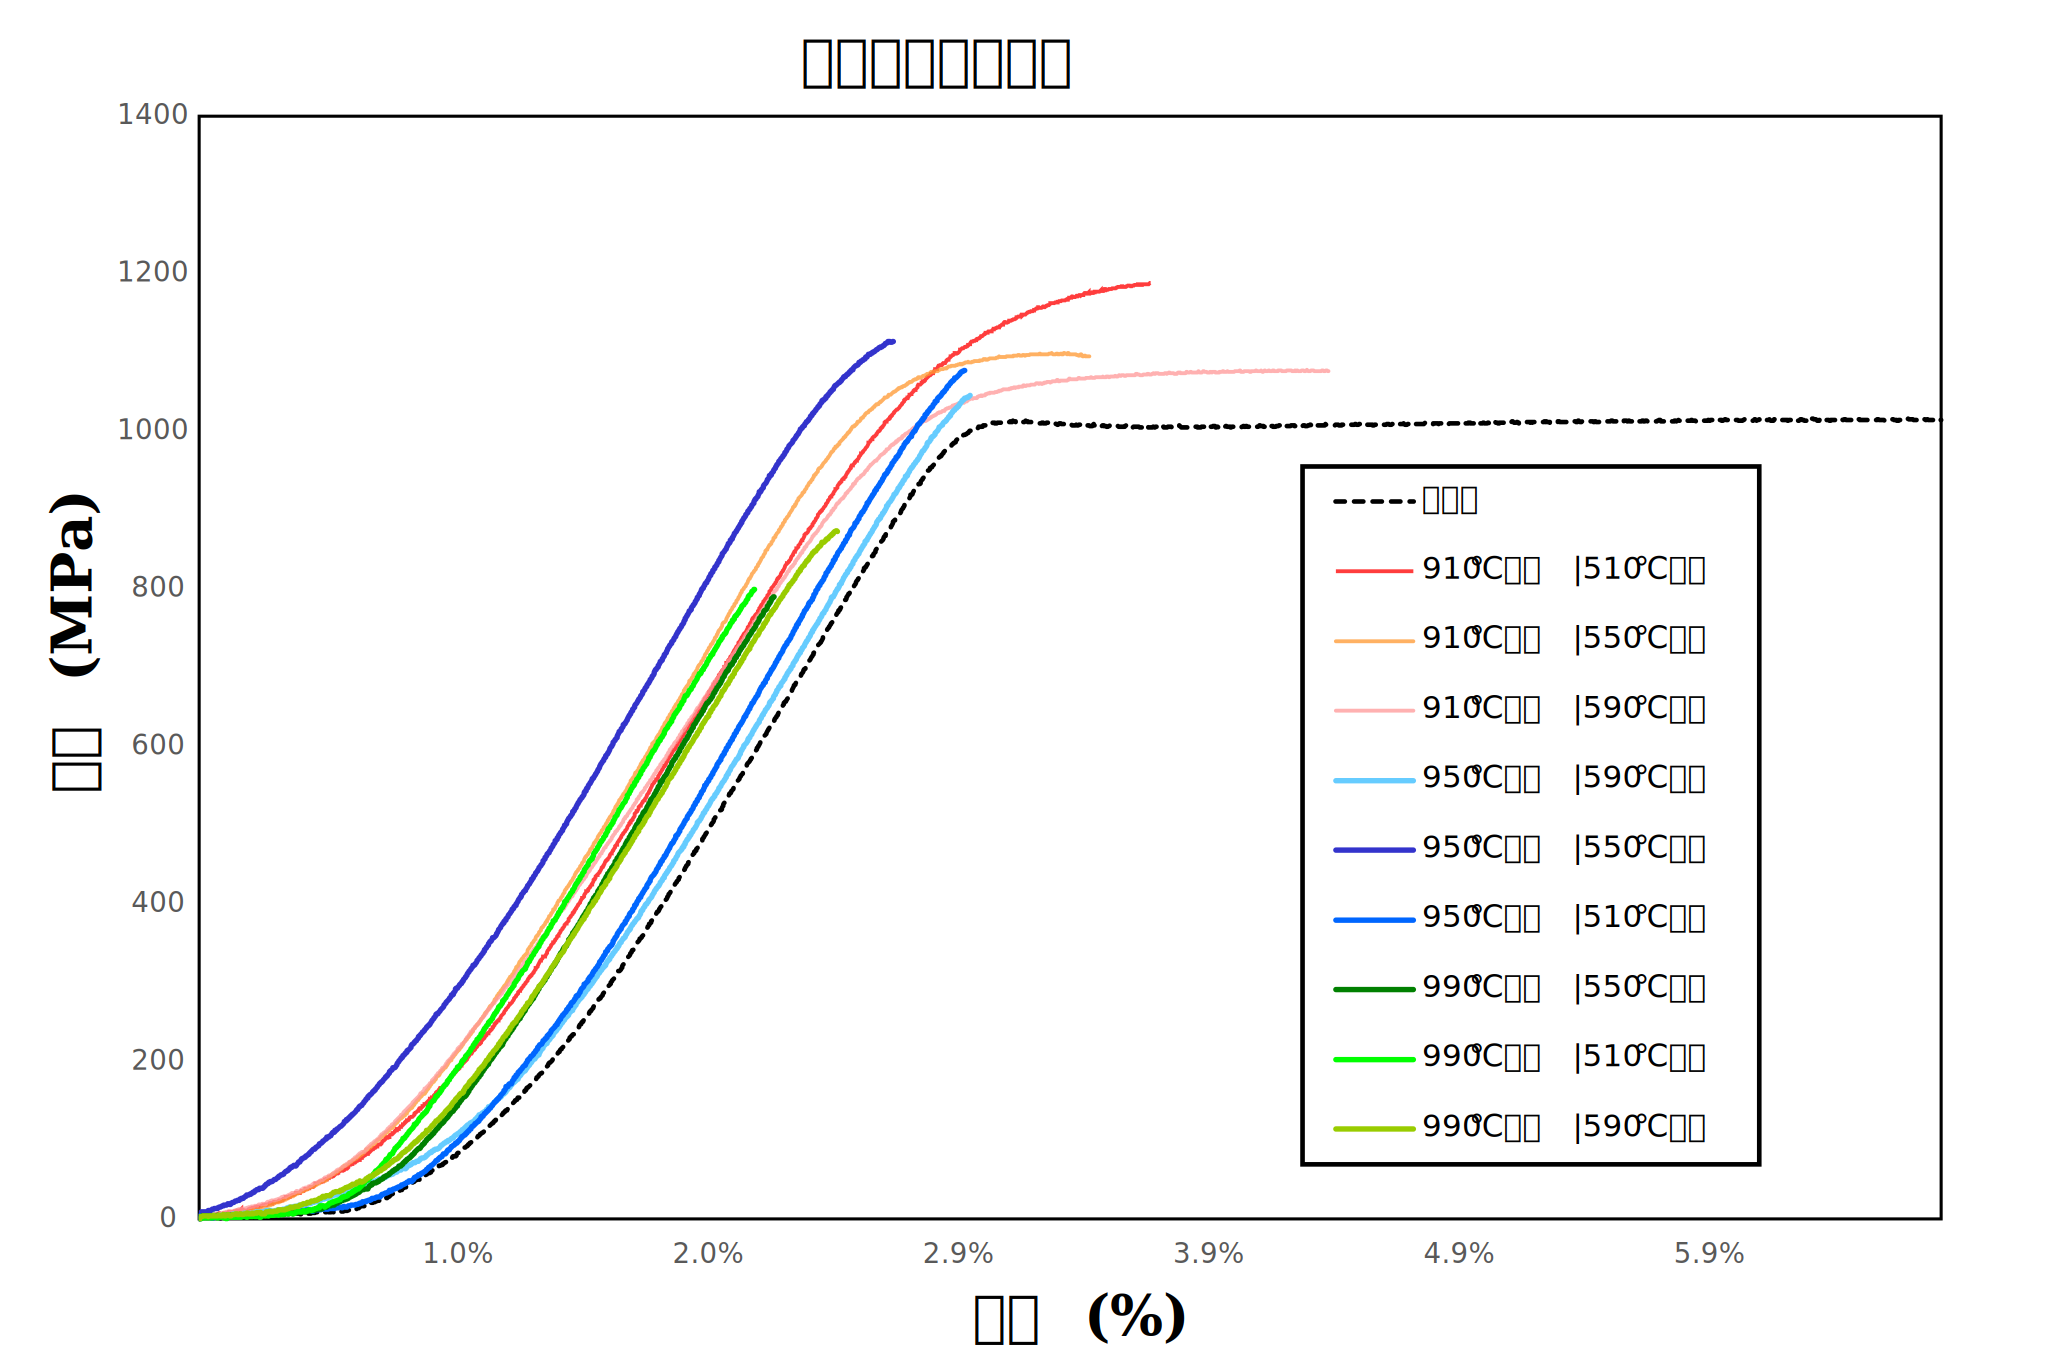
\includegraphics[width=0.99\linewidth]{pic/试样应力应变曲线汇总.pdf}
	\caption{试样应力应变曲线汇总}
	\label{fig:试样应力应变曲线汇总}
\end{figure}

\begin{table}[htbp]
	\centering
	\caption{\ti 合金的力学性能实验结果}
	\label{sec:mystrength}
		\begin{tabular}{ccc}
			\toprule
			实验编号&$ R_m $/Mpa&$ R_{p0.2} $/Mpa \\
			\midrule
			1 & 950 & 866\\
			2 & 946 & 872\\
			3 & 976 & 884\\
			4 & 988 & 894\\
			5 & 990 & 920\\
			6 & 972 & 886\\
			7 & 966 & 820\\
			8 & 978 & 849\\
			9 & 959 & 836\\
			\bottomrule
		\end{tabular}
\end{table}
\newpage
\section{显微组织表征实验设备}
试验期间用来观察组织和分析相结构的检测方法,主要包括光学显微镜 (OM)、扫描式电子显微镜 (SEM)、X射线衍射分析 (XRD)以及透射式电子显微镜 (TEM)等。

将固溶与时效后的试件进行线切割截取显微组织分析试样,截取后的试样进行 150\#、400\#、1000\#、1500\#、2000\#、2500\#金相砂纸磨制,对磨制后的试样采用 0.05umSiO2抛光液在抛光机上进行抛光,去除试样表面的划痕或杂质颗粒,经抛光后的试样采用$ HF:HNO3:H2O=2:4:94 $的Kroll试剂进行腐蚀。腐蚀后的试样分别采用光 学显微镜(OM)、扫描电子显微镜(SEM)对其微观形貌进行观察。

\section{式样的显微组织表征与结果分析}
三种不同固溶温度得到的试样组织如下:
\begin{figure}[h!]
	\centering
	\includegraphics[width=0.7\linewidth]{pic/demo-mico}
	\caption{不同热处理工艺下 TC4 钛合金的显微组织}
	\label{fig:demo-mico}
\end{figure}
	\chapter{综合分析}


本设计采用固溶-时效工艺对合金进行处理,。

固溶处理的目的是为了使合金在高温状态下内部合金元素发生充分扩散,促使 一定体积分数的 α→β 转变,然后在较快冷却条件下抑制连续冷却过程中 β→α 转变, 从而获得 α′相、α′′相以及 β′相等亚稳定相,为后期的时效处理提供良好的组织状态。 时效处理的目的是通过将固溶处理过程中得到的亚稳定相加热到一定温度进行等温 处理,在热力学的条件下,促使亚稳定相向稳定状态转变,产生细小弥散分布的析 出相,从而对钛合金起到强化作用。

TC4 钛合金在稳定状态下含有少量的 β 相,β 相的存在使其具有热处理强化的能 力。由\ref{fig:tc4change}可知,固溶处理过程中固溶温度对固溶后的亚稳定相种类起决定作 用,不同固溶温度下 α 与 β 相的平衡体积分数不同,造成 β 相中合金元素含量不同, 从而在快速冷却过程中产生不同的亚稳定相。
\begin{figure}[h!]
	\centering
	\includegraphics[width=0.7\linewidth]{pic/tc4change}
	\caption{钛合金在淬火过程中的亚稳定相及马氏体转变温度}
	\label{fig:tc4change}
\end{figure}
\section{固溶处理的影响}
\subsection{固溶温度对组织性能的影响}
钛合金在进行固溶处理时,固溶温度对其在高温平衡状态下 α 相体积分数具有 决定性作用。
选取经 910°C、950°C与 990°C分别固溶 1h 水冷的显微 组织进行观察,如所示。可以看出在 α+β 两相区进行固溶后水冷,显微组织 为初生的等轴 α 相与细针 α′状马氏体组成;由图 3-4 e)所示,在 β 单相区进行固溶后 水冷,显微组织为粗大的原始 β 晶粒内部分布着单一的细针状马氏体,马氏体在晶 内交错排列,夹角成 60 度或 90 度。

\begin{figure}[h!]
	\centering
	\includegraphics[width=0.7\linewidth]{pic/demo-不同固溶温度的影响}
	\caption{不同固溶温度下的组织}
	\label{fig:demo-}
\end{figure}


\subsection{冷却方式对组织性能的影响}
图 3-2 为 TC4 钛合金经 950°C保温 1 小时分别进行油冷和水冷后的显微组织形 貌,从图中可以看出,油冷后组织主要是由初生等轴 α 相和 β 转变组织组成的双态 组织,水冷后组织主要是由等轴初生 α 相和针状马氏体组成。TC4 钛合金在加热过 程中,随着温度的升高,α 相逐渐转变为 β 相,当加热温度未高于相变点温度时,高 温状态下组织由未溶解的初生等轴 α 相和 β 相构成。在连续冷却过程中,未溶解的 初生等轴 α 相进行扩散型长大,由于油冷的冷却速率小于水冷,初生等轴 α 相的长 大时间要多于水冷,造成油冷后初生等轴 α 相的晶粒尺寸大于水冷。利用 XRD 分析 了固溶后经不同冷却方式后的相组成,如图 3-3 所示。

\begin{figure}[h!]
	\centering
	\includegraphics[width=0.7\linewidth]{pic/demo-油冷与水冷的对比}
	\caption{不同冷却方式下的 TC4 钛合金显微组织}
	\label{fig:demo-油冷与水冷}
\end{figure}

TC4 钛合金 950°C固溶分别经油冷和 水冷后,相的组成存在较大差异,油冷时的冷却速率较低,高温 β 相中的合金元素 在冷却过程中发生扩散,进行扩散型相变,导致次生 α 相在初生 α 与 β 相界面处形 核,并向 β 相晶内长大,生成 α 片层与 β 片层相间的 β 转变组织,最终相的构成包 α 相与 β 相;水冷时的冷却速率极快,冷却过程基本在瞬间完成,导致 β→α 的扩散型 相变来不及发生,β 相通过晶格切变的形式进行原子集体的、有规律的近程迁移,生 成 α′马氏体,最终相的构成包含 α 相与 α′相,没有发现 β 相存在。


\section{时效处理的影响}
\subsection{时效温度对组织性能的影响}

时效处理时组织转变的物质基础是:固溶或者退火处理得到的马氏体$ \alpha^{\prime} $相和亚稳$ \beta $相,这两种相是热力学上不稳定的物质,加热时会分解。

固溶在高温下将大量的 $\alpha$ 相转变 为 $\beta$ 相, 然后进行快速冷却, 可以防止过多的 $\beta$ 相 转变为 $\alpha$ 相。在保留了高温 $\beta$ 组织的同时, 发生了马氏体相变,部分 $\beta$ 相转变为不稳定的 $\alpha^{\prime}$ 相和 $\alpha^{\prime \prime}$ 相, 为时效相转变提供了良好的组织\cite{ xinsheweiGuanyutaihejinrechulihexichuxiangdetaolun2006,zouhaibeiTC4taihejinrechuliqianghuagongyijixiangbianhangweiyanjiu2019a}。时效处理通过对亚稳定组织低温热处理, 促使亚稳定组织 $\beta$ 相、$ \alpha  ^{\prime}$相及 $ \alpha  ^{\prime\prime}$相转变为细小、室温稳定的等轴组织与片层组织,以起到弥散强化作用,改善组织的塑性和韧性。常见的组织为\cite{zhanghaoyinGurongShixiaoduiTC4taihejinzuzhihelixuexingnengdeyingxiang2014}: $ \alpha  ^{\prime}$相、$ \alpha  ^{\prime}$相脱溶出来的等轴$ \alpha$相与$ \beta $相、变粗大的$ \alpha $相、 $ \beta $相。

对于固溶-时效组合处理工艺而言,固溶后TC4钛合金中马氏体仍保持$ \alpha $相软而韧的性能,在随后进行时效强化可以使得马氏体分解,获 得 弥 散 的轴$ \alpha+\beta $组织,从而进一步提高其抗拉强度。 但随 着 时 效 温度的升高,伸长率会逐 渐 上 升,抗拉强度则呈下降趋势。当时效温度过高时,组织会粗化,使合金的塑性、韧性下降\cite{guxiaohuiCuihuoShixiaowenduduiTC4taihejinzuzhihelixuexingnengdeyingxiang2011}。

时效处理温度主要影响\ti 合金中次生$ \alpha $的尺寸,Sauer\cite{sauerThermomechanicalProcessingHigh2001}等人研究发现\ti 合金中沿着$ \beta $晶界形成的连续$ \alpha  $片层组织对合金的机械加工性能有负面影响,等轴$ \beta $相越大,负面作用越强烈;经过重结晶等匀质化处理后,可以调整$ \alpha $相的体积分数,进而改善性能。鲁媛媛、马保飞\cite{luyuanyuanShixiaochuliduiTC4taihejinweiguanzuzhihelixuexingnengdeyingxiang2019}等人研究了970℃固溶处理之后,在不同固溶温度下合金的组织,研究发现,当时效温度在 $450{ }^{\circ} \mathrm{C}$ 到 $550{ }^{\circ} \mathrm{C}$之间时 ,随温度增加,合金的强度值 逐渐增加; 但当温度大于 $600{ }^{\circ} \mathrm{C}$ 时,强度随温度增加而逐渐下降,当时效温度为 $550{ }^{\circ} \mathrm{C}$ 时,合金的强度最高。李露\cite{lilouGurongshixiaoduiTC4hejinzuzhiyujixiexingnengdeyingxiang2014}研究发现TC4合金的硬度随时效温度的升高而下降,当 固溶快冷组织为亚稳 的 $\beta 、 \alpha^{\prime} 、 \alpha^{\prime\prime}$ 相,时 时效过程分解产物为弥散的 $\alpha$ 和 $\beta$ 相, 而且时效温度越高, 分解越充分, 硬度越低。

顾晓辉\cite{guxiaohuiCuihuoShixiaowenduduiTC4taihejinzuzhihelixuexingnengdeyingxiang2011}人研究发现同等条件下,时效温度越低,$ \alpha^{\prime} $转变得到的$ \alpha+\beta  $相组织越细小,越弥散;当固溶温度提高时,组织变粗,这与二次$ \beta $相的分解密切相关,当初生$ \alpha $相的尺寸较大时,随时效温度升高,析出的$ \alpha $相会与初生$ \alpha $相聚集长大,发生球化。

在时效后的得到等轴组织和双态组织中,均含有一定量的等轴初 生 $\alpha$ 相。而拉伸变形通常是在等轴初生 $\alpha$ 相的某晶粒开始滑移,裂纹往往在在相界面上产生。 变形过程中,随着变形量的增大, 初生$\alpha$ 晶粒会产生更多的滑移, 并 向周围的 $\beta$ 转变组织扩展, 导致空洞形核、和扩展变慢迟, 断裂前将产生更大的变形, 从而获更高的塑性\cite{yekangyuanRechuliduiTC4taihejinduanjianzuzhihexingnengdeyingxiang2022}。

\section{结论}


	\backmatter
	\listoffigures
	\listoftables
	\clearpage
	\phantomsection
	\addcontentsline{toc}{chapter}{参考文献}
	\bibliography{ciiiiiiiiite}
	\chapter{附录}
附录编号依次编为附录1,附录2。附录标题各占一行,按一级标题编排。每一个附录一般应另起一页编排,如果有多个较短的附录,也可接排。附录中的图表公式另行编排序号,与正文分开,编号前加“附录1-”字样。

 每位学生须阅读一定的专业外文资料(专著、期刊、学位论文、论文集、报纸文章、报告、标准、专利、教材、网络资料等),通过文献查阅与阅读,进一步提高使用外文的能力,熟悉本专业的几种主要外文书刊,了解毕业论文(设计)课题的国内外信息与动态。

 翻译的原文应该是来源于学校认可的数据库资源,且是与毕业论文(设计)题目密切相关的资料。译文字数3000字符左右,要求译文与原文内容相符。

 译文要求:
 \begin{enumerate}
 	\item (1)标题 (2)署名 (3)翻译正文 (4)外文著录
 	\item 附被翻译文字资料原件的复印件
 \end{enumerate}

	\chapter{致谢}
致谢:对于毕业论文(设计)的指导教师,对毕业论文(设计)提过有益的建议或给予过帮助的同学、同事与集体,都应在论文的结尾部分书面致谢,言辞应恳切、实事求是。应注明受何种基金支持(没有可不写)。
%	\includepdf{致谢}
%	\includepdf{指导老师评议书}
%	\includepdf{评阅老师评议书
%	\includepdf{答辩委员会评议书}}

%附件:
%  1.新疆大学本科毕业论文(设计)工作进展情况记录表
%	2.中期检查表
%	3.毕业论文(设计)答辩记录
%	4.程序与附件
\end{document}


